%\documentclass[preprint,5p,twocolumn,11pt,sort&compress]{article}
%\usepackage{amssymb}
%\usepackage{amsthm}
%\usepackage{tabularx}
%\usepackage{graphicx}
%\usepackage{epsfig}
%\usepackage{textcomp}
%\usepackage{subfigure}
%\usepackage{natbib}
%\usepackage[colorlinks,linkcolor=red,anchorcolor=blue,citecolor=blue]{hyperref}
%\usepackage{color,soul}
%\usepackage{multirow}
%\usepackage{ctex}
%
%%\bibliographystyle{elsarticle-num}
%
%\begin{document}
%
%\title{镍基高温合金热梯度机械疲劳条件下的寿命预测}
%
%\author{Jingyu SUN\fnref{label1}}
%\author{Huang YUAN\corref{cor1}\fnref{label1}}
%
%
%\begin{abstract}
%Turbine components are generally under mechanical and thermal loads. Recent works confirm significant effects of thermomechanical loads to fatigue life assessment. In the present work, extensive experiments are performed for a nickel-based superalloy under both iso-thermal and thermo-mechanical loading conditions to quantify influence of thermal phase angle and loading non-proportionality. Based on experimental data a thermomechanical loading parameter is introduced to assess fatigue failure. The thermomechanical fatigue life can be calibrated based on the present concept reasonably.
%\end{abstract}
%
%%\include{debut}
%\begin{keyword}
%% keywords here, in the form: keyword \sep keyword
%Thermomechanical Fatigue (TFM) \sep Multi-Axial Fatigue \sep Fatigue Damage \sep Fatigue Life \sep Nickel-based super alloy
%
%% PACS codes here, in the form: \PACS code \sep code
%% \PACS
%\end{keyword}
%
%
%% main text
%\section{Introduction}
%\section{Experiments}
%\subsection{Material specification}
%\section*{Acknowledgement:}
%
%\bibliographystyle{unsrt}            % bibliography style
%%\bibliographystyle{plain}            % bibliography style
%\bibliography{bibliography}          % personal bibliography file
%
%\end{document}

\documentclass{article}
\usepackage{hypernat}              % ensure cooperation of natbib and hyperref
\usepackage{booktabs}
\usepackage[below]{placeins}
\usepackage{fancyhdr}
\usepackage{mdwlist}
\usepackage{indentfirst}
\usepackage[Symbol]{upgreek}
\usepackage{bm}
\usepackage{framed}
\usepackage{threeparttable}
\usepackage{overpic}
\usepackage{booktabs}
\usepackage{ctex}

\graphicspath{{F:/Cloud/GitHub/tgmf/figs/}{F:/Cloud/GitHub/doctor/figs/}{F:/Cloud/GitHub/doctor/figs/python/}{F:/Cloud/GitHub/doctor/figs/ppt/}{F:/Cloud/GitHub/doctor/figs/svg/}{F:/Cloud/GitHub/doctor/figs/sem/}{F:/Cloud/GitHub/doctor/figs/test/}}

\begin{document}
\title{镍基高温合金热梯度机械疲劳条件下的寿命预测}



\author{袁荒,孙经雨}
\date{\today}
\maketitle
\tableofcontents

\section*{摘要}
研究了镍基高温合金热梯度机械疲劳条件下的疲劳寿命,与恒温疲劳试验寿命和无温度梯度的热机械疲劳寿命进行比较,
带有温度梯度的热机械疲劳寿命要明显降低。
同时考虑相位对热梯度机械疲劳寿命的影响,在低周疲劳的情况下,同相位的热梯度机械疲劳寿命要明显低于反相位的寿命。
同时研究了涂覆热障涂层对镍基高温合金样品的热梯度机械疲劳性能的影响。
结果表明,随热障涂层可以有效的提高材料的热梯度机械疲劳寿命。
通过有限元计算,确定试件在每个循环内的温度场分布,同时基于循环塑性本构方程计算当前温度场下的应力应变曲线。
考虑到温度梯度,建立了一个涂覆热障涂层高温合金样品的热梯度机械疲劳寿命预测模型。

\section{概述}
热障涂层涂覆于航空发动机和燃气轮机高温部件表面,具有防止高温腐蚀、延长热端部件使用寿命、提高发动机功率和减少燃油消耗等优点。通
常典型的热障涂层包括表面陶瓷层(TC:top coat)和金属粘结层(BC:bond coat)。在服役过程中,粘结层会发生氧化,在粘结层和陶瓷层界面形成厚度为1~10$\mu$m的热生长氧化物(TGO:thermally grown oxide)。TGO的形成是一个体积膨胀过程,界面会限制这种体积变化,因而在TGO内部会随之产生应力。而且,陶瓷层与金属基底的热膨胀系数相
差较大,在热循环过程中会在热载荷的作用下产生较大的热应力,从而在界面缺陷处引起应力集中,促进裂纹的萌生与扩展。
\section{试验}
发动机涡轮叶片主要采用气膜冷却和内部流冷却,轮盘通常采用内部二次流冷却。
服役过程中,涡轮叶片不仅受到较大的交变载荷,而且在叶片表面和内部分别受到高温高压燃气的冲击和冷却气体的作用,这样涡轮叶片就遭受载荷和温度同时变化带来的热机械疲劳损伤。
此外,为了增强发动机冷却效果,提高发动机效率,先进的航空发动机和燃气轮机热端涡轮叶片多为薄壁多孔结构。
因此,我们设计了薄壁圆管试件来模拟零件的冷却结构,同时试件外壁涂覆有热障涂层。
在内部冷却气体作用下,试件内表面与外表面之间会产生很大的温度梯度,同时导致额外的应力,在热表面上表现为多轴压缩载荷,而在冷却表面上表现为多轴拉伸载荷。

对于薄壁圆管试件,我们可选择的加热方式有电阻炉、电磁感应、火焰喷射和辐射。
电阻炉的优点在于温度稳定性好,但实际发动机启动阶段升温过程只需要几十秒钟的时间,而且降温也相当迅速,采用电阻炉无法实现试件的快速升温和降温。
电磁感应加热的优点在于加热效率高,试件升温迅速,通常热机械疲劳试验采用高频电磁感应设备进行加热,其中高频电磁感应加热厚度约为2mm,这意味着试件的内外表面是同时加热的,在内部冷却过程中,不利于产生内外表面的温度梯度,同时电磁感应方式只会对内部金属层加热,使得内部金属层温度高于外部陶瓷层温度,这不符合热障涂层构件实际工作状态下的温度分布。
火焰喷射的优点在于接近真实发动机涡轮叶片的工作环境,但火焰的稳定性差,火焰形状难以控制,很难形成均匀的温度场。

因此我们为热梯度机械疲劳(TGMF)测试设计开发了聚光辐射加热系统。
该系统包括16根卤素灯管,灯丝的直径小于0.5mm,因此每根灯丝可以被抽象为一个线光源。
每根灯管对应一面反射镜,反射镜的几何形状为椭圆柱面,每根灯管位于其对应的椭圆柱面其中一个焦点,试件位于所有椭圆柱面的公共焦点,通过镜面反射将光线聚焦在试件表面进行加热。
通过聚光辐射的方法加热试件外表面,同时内表面通过压缩空气冷却来实现温度梯度。
该系统可以在空心试件表上实现受控的温度梯度循环,同时施加机械载荷,适用于金属和非金属材料。


\begin{figure}[!htp]
\centering{\includegraphics[width=12cm]{Radiation_Furnace2.pdf}}
\caption{TGMF试样示意图.}
\label{Fig:Radiation_Furnace2}
\end{figure}

\begin{figure}[!htp]
\centering{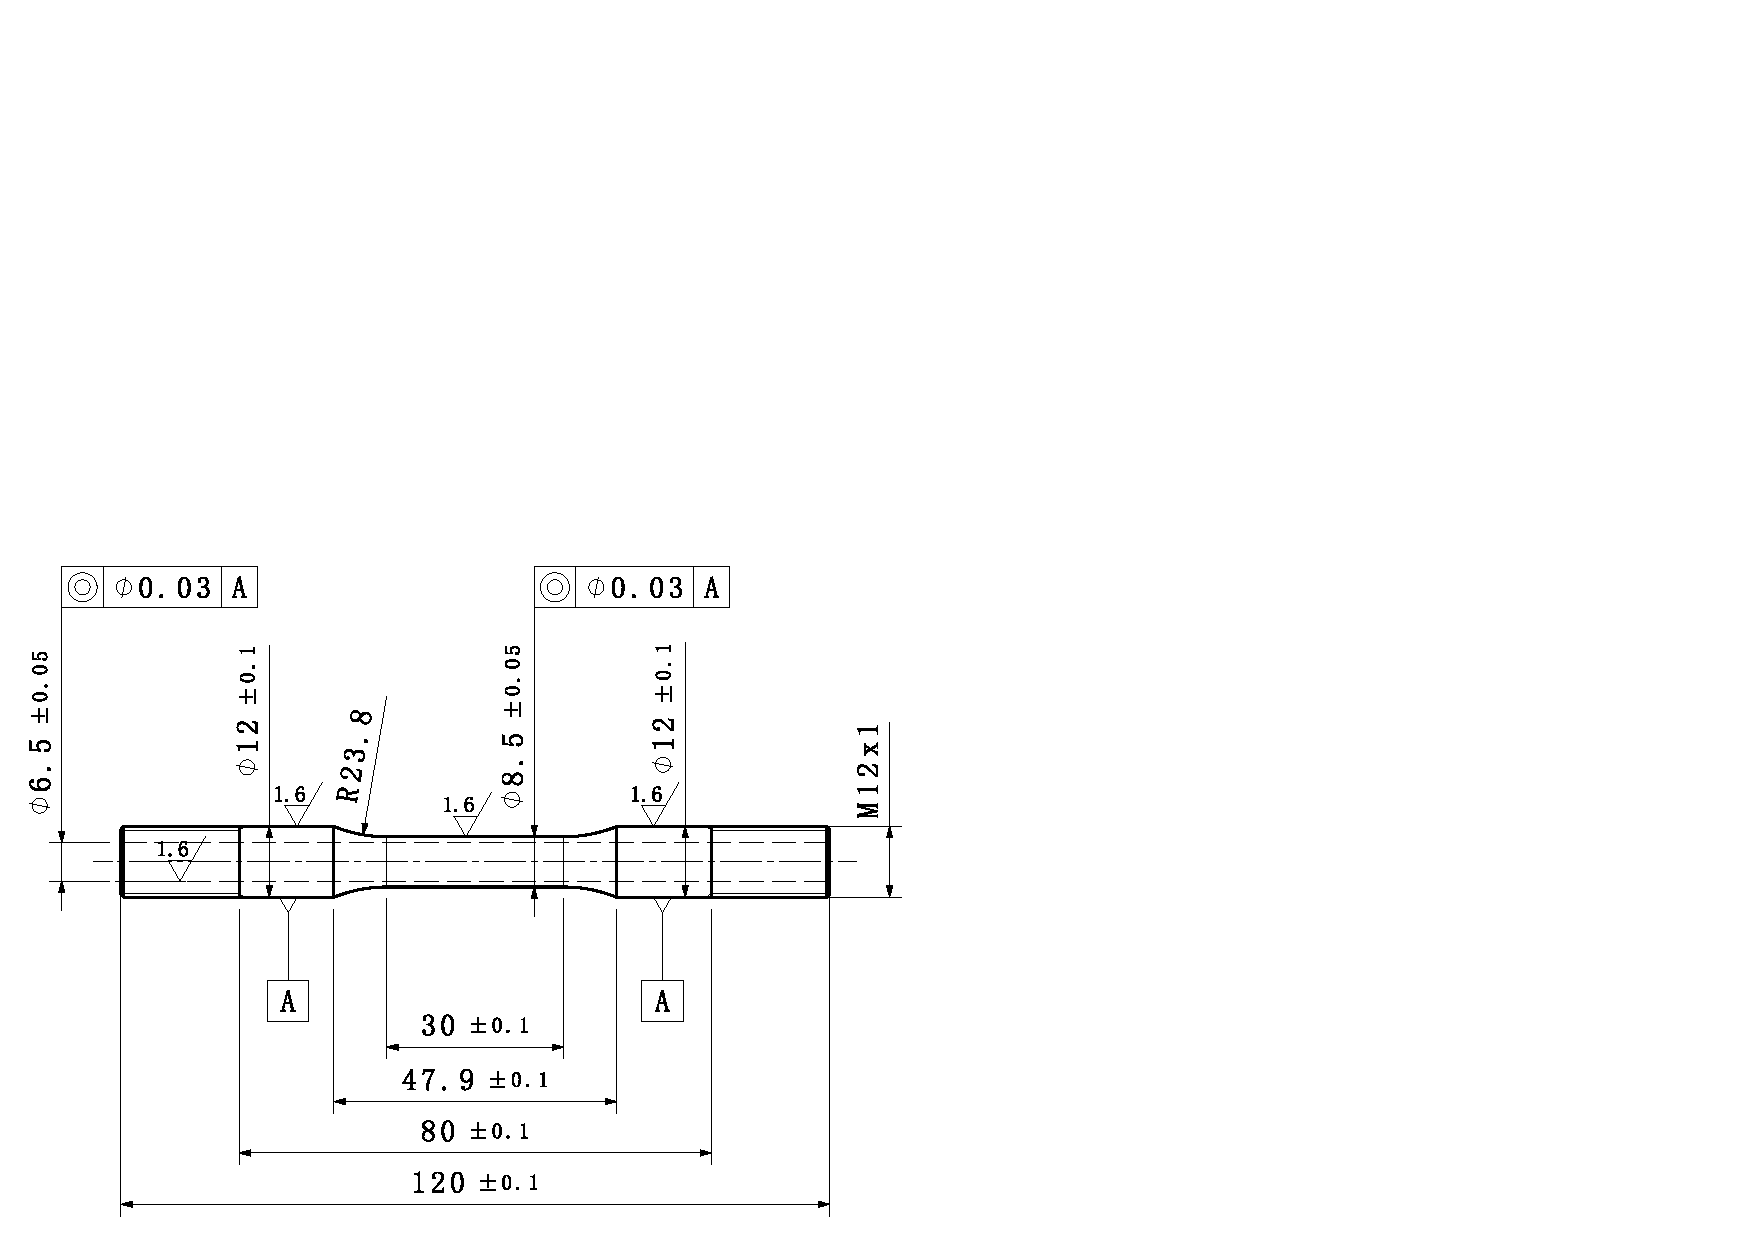
\includegraphics[width=12cm]{IN718_Axial_Specimen_TGMF.pdf}}
\caption{TGMF试样示意图.}
\label{Fig:Specimen}
\end{figure}
\section{试验结果}

\begin{table}[htbp]
  \centering
  \caption{650$^{\circ}$C恒温疲劳试验、TMF与TGMF试验结果.}
    \begin{tabular}{llllll}
    \toprule
    Test Type & $\pm \varepsilon _m$ & $\varepsilon _{eq}$ & $\dot \varepsilon _{eq}$ & $\theta_{T-\varepsilon}$ & $N_f$ \\
          & [\%]  & [\%]  & [s$^{-1}$] & [$^\circ$] &  \\
    \midrule
    IF & 1.00  & 1.00  & $1\times 10^{-3}$ & -     & 131 \\
          & 0.80  & 0.80  & $1\times 10^{-3}$ & -     & 326 \\
          & 0.70  & 0.70  & $1\times 10^{-3}$ & -     & 592 \\
          & 0.60  & 0.60  & $1\times 10^{-3}$ & -     & 1336 \\
          & 0.50  & 0.50  & $1\times 10^{-3}$ & -     & 8449 \\
          & 0.45  & 0.45  & $1\times 10^{-3}$ & -     & 15497 \\
          & 0.40  & 0.40  & $6.4\times 10^{-3}$ & -     & 130585 \\
    \midrule
    TMF-IP & 1.00  & 1.00  & $2.22\times 10^{-4}$ & 0     & 58 \\
          & 0.80  & 0.80  & $1.78\times 10^{-4}$ & 0     & 176 \\
          & 0.70  & 0.70  & $1.56\times 10^{-4}$ & 0     & 248 \\
          & 0.60  & 0.60  & $1.33\times 10^{-4}$ & 0     & 1297 \\
    \midrule
    TMF-OP & 1.00  & 1.00  & $2.22\times 10^{-4}$ & 180   & 209 \\
          & 0.80  & 0.80  & $1.78\times 10^{-4}$ & 180   & 303 \\
          & 0.70  & 0.70  & $1.56\times 10^{-4}$ & 180   & 429 \\
          & 0.65  & 0.65  & $1.44\times 10^{-4}$ & 180   & 633 \\
    \midrule
    TGMF-IP & 0.75  & 0.75  & $1.67\times 10^{-4}$ & 0     & 48 \\
          & 0.60  & 0.60  & $1.33\times 10^{-4}$ & 0     & 50 \\
          & 0.55  & 0.55  & $1.22\times 10^{-4}$ & 0     & 107 \\
          & 0.50  & 0.50  & $1.11\times 10^{-4}$ & 0     & 208 \\
          & 0.40  & 0.40  & $0.89\times 10^{-4}$ & 0     & 1066 \\
    \midrule
    TGMF-OP & 0.75  & 0.75  & $1.67\times 10^{-4}$ & 180   & 128 \\
          & 0.55  & 0.55  & $1.22\times 10^{-4}$ & 180   & 375 \\
          & 0.50  & 0.50  & $1.11\times 10^{-4}$ & 180   & 864 \\
          & 0.40  & 0.40  & $0.89\times 10^{-4}$ & 180   & 3387 \\
    \midrule
    TGMF-IP-TBC & 0.75  & 0.75  & $1.67\times 10^{-4}$ & 0     & 147 \\
          & 0.55  & 0.55  & $1.22\times 10^{-4}$ & 0     & 624 \\
    \bottomrule
    \end{tabular}%
  \label{tab:addlabel}%
\end{table}%

\begin{figure}[!htp]
\centering{\includegraphics[width=12cm]{plot_exp_fatigue_life.pdf}}
\caption{TMF与TGMF寿命比较.}
\label{Fig:plot_exp_fatigue_life}
\end{figure}


\section{微观结构}

% \begin{figure}
%   \begin{minipage}[t]{0.5\linewidth}
%   \nonumber
%     \centering
%     \includegraphics[width=6cm]{7033-1.jpg}
%     \centerline{(a)500X.}
%   \end{minipage}%
%   \begin{minipage}[t]{0.5\linewidth}
%     \centering
%     \includegraphics[width=6cm]{7033-12.jpg}
%     \centerline{(b)850.}
%   \end{minipage}
%   \caption{TC-OP.}
%   \label{Fig:MicrostructureofInconel718}
% \end{figure}

% \begin{figure}
%   \begin{minipage}[t]{0.5\linewidth}
%   \nonumber
%     \centering
%     \includegraphics[width=6cm]{7036-1.jpg}
%     \centerline{(a)$\Delta \varepsilon_{m}/2=0.5\%$.}
%   \end{minipage}%
%   \begin{minipage}[t]{0.5\linewidth}
%     \centering
%     \includegraphics[width=6cm]{7036-7.jpg}
%     \centerline{(b)$\Delta \varepsilon_{m}/2=0.5\%$.}
%   \end{minipage}

%   \begin{minipage}[t]{0.5\linewidth}
%   \nonumber
%     \centering
%     \includegraphics[width=6cm]{7046-1.jpg}
%     \centerline{(C)$\Delta \varepsilon_{m}/2=0.7\%$.}
%   \end{minipage}%
%   \begin{minipage}[t]{0.5\linewidth}
%     \centering
%     \includegraphics[width=6cm]{7046-6.jpg}
%     \centerline{(D)$\Delta \varepsilon_{m}/2=0.7\%$.}
%   \end{minipage}

%   \caption{NRP-IP.}
%   \label{Fig:MicrostructureofInconel718}
% \end{figure}

% \begin{figure}
%   \begin{minipage}[t]{0.5\linewidth}
%   \nonumber
%     \centering
%     \includegraphics[width=6cm]{7047-1.jpg}
%     \centerline{(a)500X.}
%   \end{minipage}%
%   \begin{minipage}[t]{0.5\linewidth}
%     \centering
%     \includegraphics[width=6cm]{7047-12.jpg}
%     \centerline{(b)1000X.}
%   \end{minipage}
%   \caption{TC-IP.}
%   \label{Fig:MicrostructureofInconel718}
% \end{figure}

% \begin{figure}
%   \begin{minipage}[t]{0.5\linewidth}
%   \nonumber
%     \centering
%     \includegraphics[width=6cm]{7112-1.jpg}
%     \centerline{(a)500X.}
%   \end{minipage}%
%   \begin{minipage}[t]{0.5\linewidth}
%     \centering
%     \includegraphics[width=6cm]{7112-3.jpg}
%     \centerline{(b)1000X.}
%   \end{minipage}
%   \caption{TC-IF.}
%   \label{Fig:MicrostructureofInconel718}
% \end{figure}

% \begin{figure}
%   \begin{minipage}[t]{0.5\linewidth}
%   \nonumber
%     \centering
%     \includegraphics[width=6cm]{7040-3.jpg}
%     \centerline{(a)$\Delta \varepsilon_{eq}/2=0.6\%$.}
%   \end{minipage}%
%   \begin{minipage}[t]{0.5\linewidth}
%     \centering
%     \includegraphics[width=6cm]{7040-5.jpg}
%     \centerline{(b)$\Delta \varepsilon_{eq}/2=0.6\%$.}
%   \end{minipage}
%   \caption{PRO-IP.}
%   \label{Fig:MicrostructureofInconel718}
% \end{figure}

% \begin{figure}
%   \begin{minipage}[t]{0.5\linewidth}
%   \nonumber
%     \centering
%     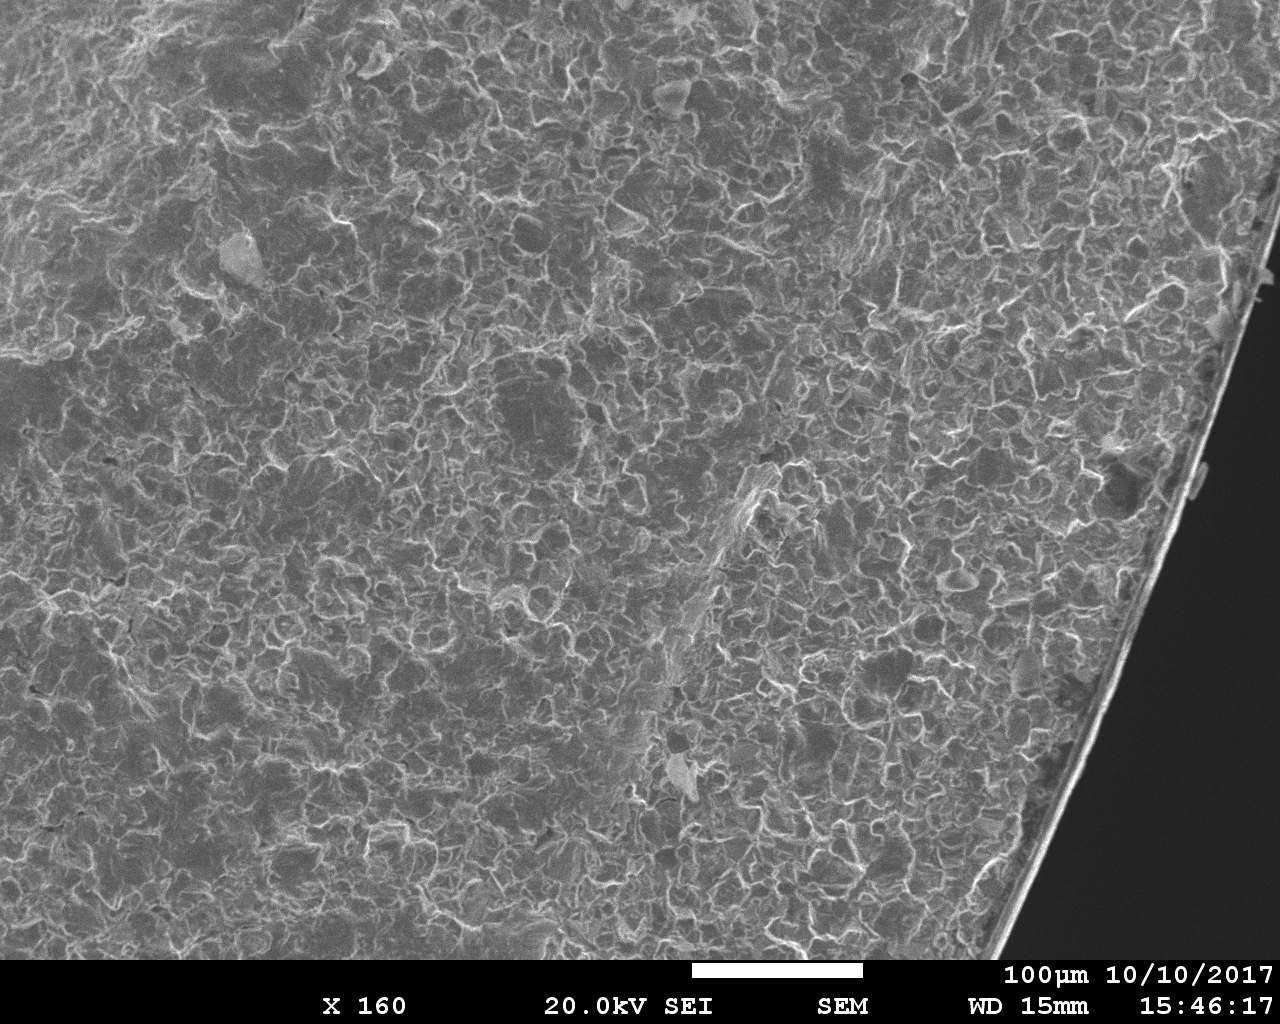
\includegraphics[width=6cm]{7206-1.jpg}
%     \centerline{(a)$\Delta \varepsilon_{eq}/2=0.55\%$.}
%   \end{minipage}%
%   \begin{minipage}[t]{0.5\linewidth}
%     \centering
%     \includegraphics[width=6cm]{7206-3.jpg}
%     \centerline{(b)$\Delta \varepsilon_{eq}/2=0.55\%$.}
%   \end{minipage}
%   \caption{TC-IP-TGMF.}
%   \label{Fig:MicrostructureofInconel718}
% \end{figure}

% \begin{figure}
%   \begin{minipage}[t]{0.5\linewidth}
%   \nonumber
%     \centering
%     \includegraphics[width=6cm]{720719.jpg}
%     \centerline{(a)$\Delta \varepsilon_{eq}/2=0.55\%$.}
%   \end{minipage}%
%   \begin{minipage}[t]{0.5\linewidth}
%     \centering
%     \includegraphics[width=6cm]{720721.jpg}
%     \centerline{(b)$\Delta \varepsilon_{eq}/2=0.55\%$.}
%   \end{minipage}

%   \begin{minipage}[t]{0.5\linewidth}
%   \nonumber
%     \centering
%     \includegraphics[width=6cm]{720932.jpg}
%     \centerline{(a)$\Delta \varepsilon_{eq}/2=0.45\%$.}
%   \end{minipage}%
%   \begin{minipage}[t]{0.5\linewidth}
%     \centering
%     \includegraphics[width=6cm]{720935.jpg}
%     \centerline{(b)$\Delta \varepsilon_{eq}/2=0.45\%$.}
%   \end{minipage}

%   \caption{TC-OP-TGMF.}
%   \label{Fig:MicrostructureofInconel718}
% \end{figure}

% \begin{figure}
%   \begin{minipage}[t]{0.5\linewidth}
%   \nonumber
%     \centering
%     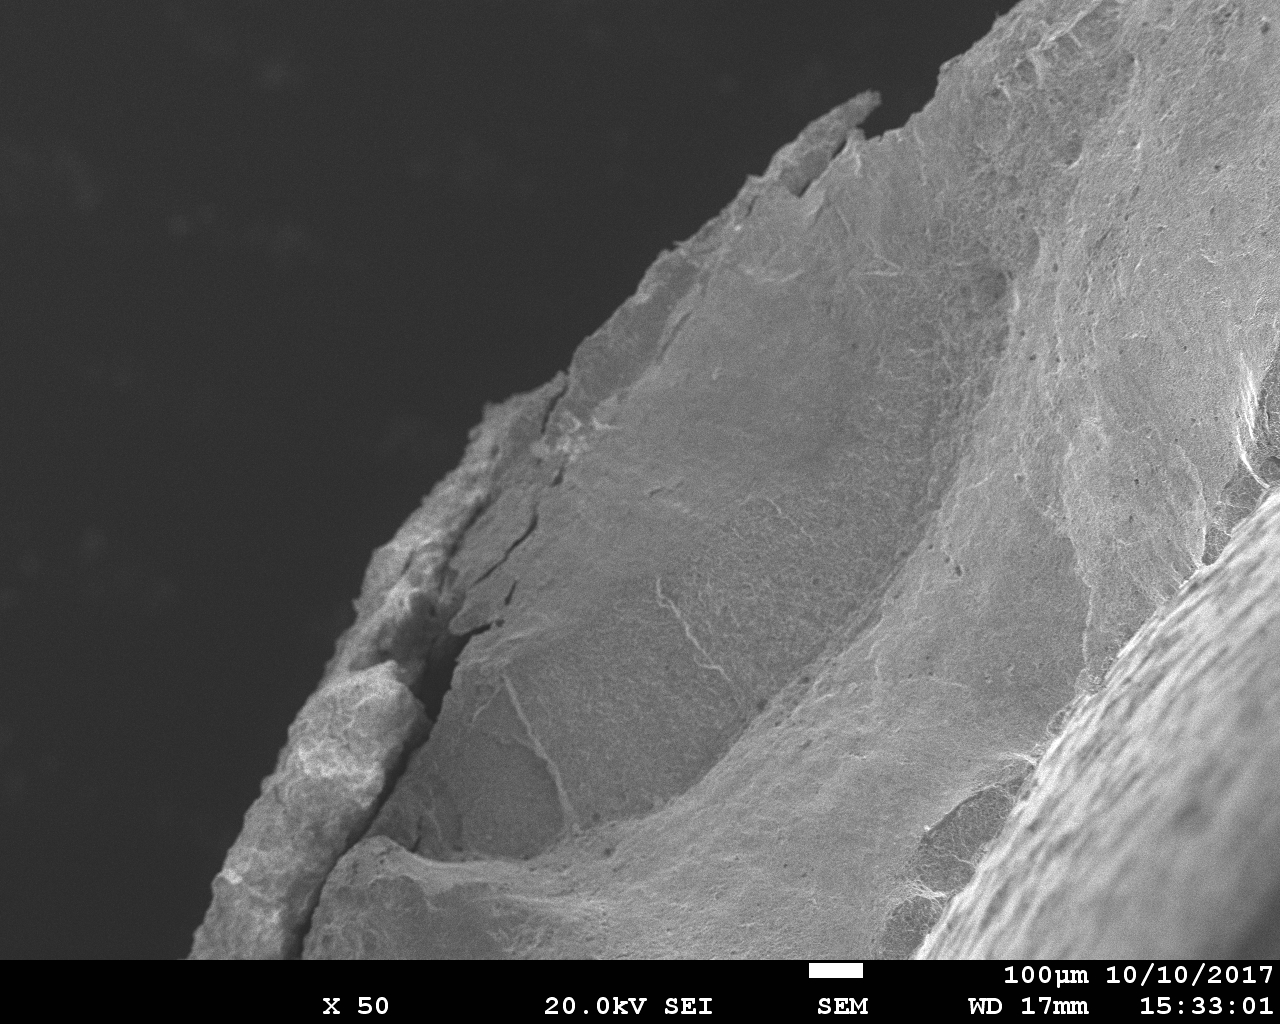
\includegraphics[width=6cm]{7301-7.jpg}
%     \centerline{(a)$\Delta \varepsilon_{eq}/2=0.55\%$.}
%   \end{minipage}%
%   \begin{minipage}[t]{0.5\linewidth}
%     \centering
%     \includegraphics[width=6cm]{7301-4.jpg}
%     \centerline{(b)$\Delta \varepsilon_{eq}/2=0.55\%$.}
%   \end{minipage}

%   \begin{minipage}[t]{0.5\linewidth}
%   \nonumber
%     \centering
%     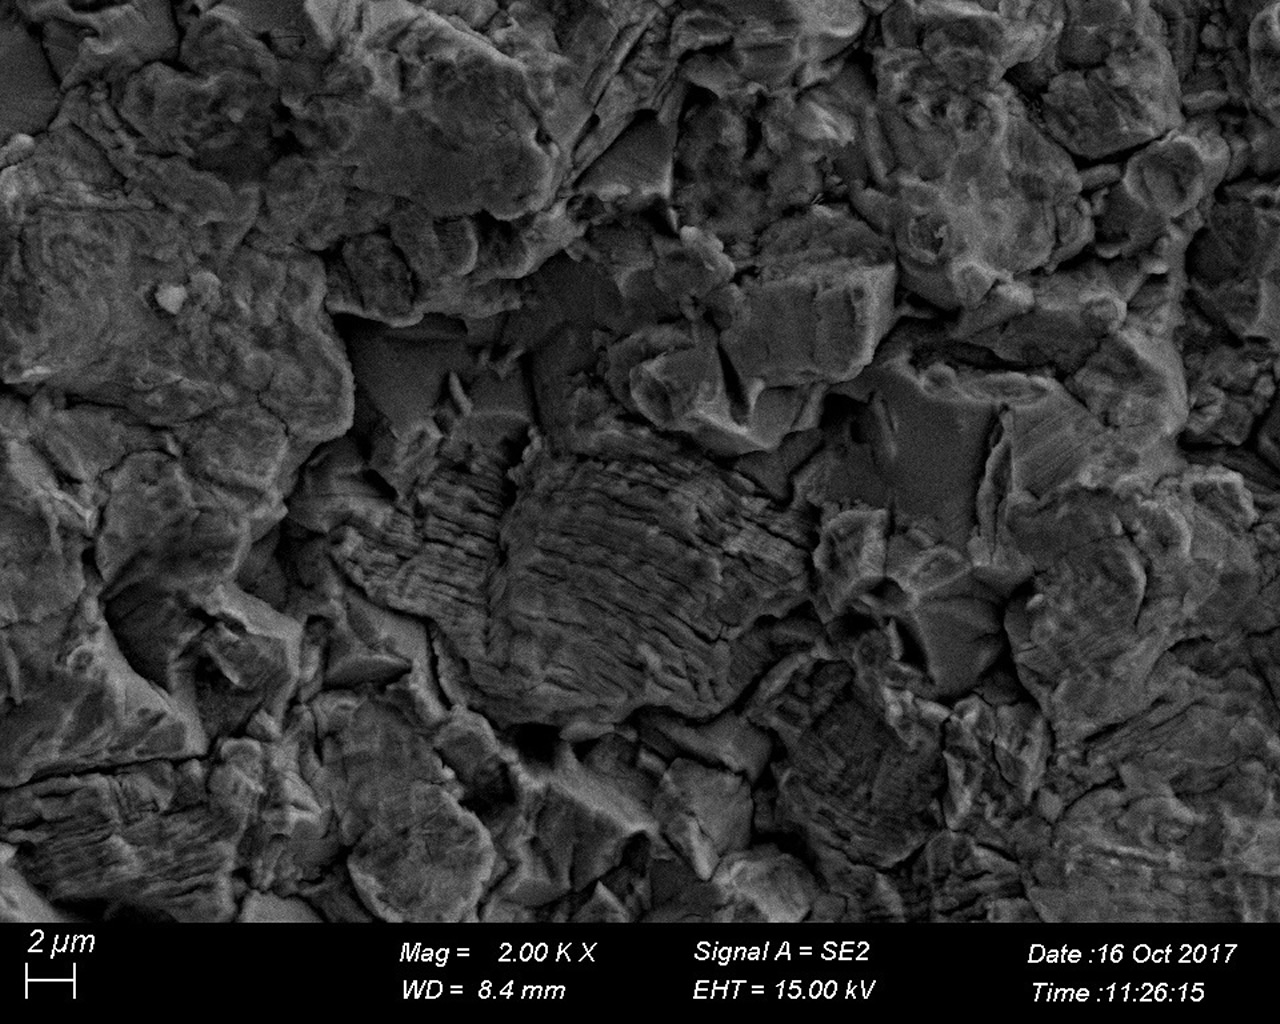
\includegraphics[width=6cm]{730109.jpg}
%     \centerline{(a)$\Delta \varepsilon_{eq}/2=0.55\%$.}
%   \end{minipage}%
%   \begin{minipage}[t]{0.5\linewidth}
%     \centering
%     \includegraphics[width=6cm]{730116.jpg}
%     \centerline{(b)$\Delta \varepsilon_{eq}/2=0.55\%$.}
%   \end{minipage}

%   \caption{TC-IP-TGMF-TBC.}
%   \label{Fig:MicrostructureofInconel718}
% \end{figure}

% \begin{figure}
%   \begin{minipage}[t]{0.5\linewidth}
%   \nonumber
%     \centering
%     \includegraphics[width=6cm]{7112-4.jpg}
%     \centerline{(a)TC-IF-650$^{\circ}$ $\Delta \varepsilon_{eq}/2=0.45\%$.}
%   \end{minipage}%
%   \begin{minipage}[t]{0.5\linewidth}
%     \centering
%     \includegraphics[width=6cm]{7047-7.jpg}
%     \centerline{(b)TC-IP $\Delta \varepsilon_{eq}/2=0.7\%$.}
%   \end{minipage}

%   \begin{minipage}[t]{0.5\linewidth}
%   \nonumber
%     \centering
%     \includegraphics[width=6cm]{7033-11.jpg}
%     \centerline{(c)TC-OP $\Delta \varepsilon_{eq}/2=0.65\%$.}
%   \end{minipage}%
%   \begin{minipage}[t]{0.5\linewidth}
%     \centering
%     \includegraphics[width=6cm]{7040-5.jpg}
%     \centerline{(d)PRO-IP $\Delta \varepsilon_{eq}/2=0.6\%$.}
%   \end{minipage}

%   \begin{minipage}[t]{0.5\linewidth}
%     \centering
%     \includegraphics[width=6cm]{7036-3.jpg}
%     \centerline{(e)NPR-IP $\Delta \varepsilon_{eq}/2=0.5\%$.}
%   \end{minipage}%
%   \begin{minipage}[t]{0.5\linewidth}
%     \centering
%     \includegraphics[width=6cm]{7046-8.jpg}
%     \centerline{(f)NPR-IP $\Delta \varepsilon_{eq}/2=0.7\%$.}
%   \end{minipage}
%   \caption{Observation of fatigue striations on fractures surface.}
%   \label{Fig:MicrostructureofInconel718}
% \end{figure}

% \begin{figure}
%   \begin{minipage}[t]{0.5\linewidth}
%   \nonumber
%     \centering
%     \includegraphics[width=6cm]{720935.jpg}
%     \centerline{(d)TC-OP-TGMF $\Delta \varepsilon_{eq}/2=0.50\%$.}
%   \end{minipage}%
%   \begin{minipage}[t]{0.5\linewidth}
%     \centering
%     \includegraphics[width=6cm]{720721.jpg}
%     \centerline{(c)TC-OP-TGMF $\Delta \varepsilon_{eq}/2=0.55\%$.}
%   \end{minipage}

%   \begin{minipage}[t]{0.5\linewidth}
%   \nonumber
%     \centering
%     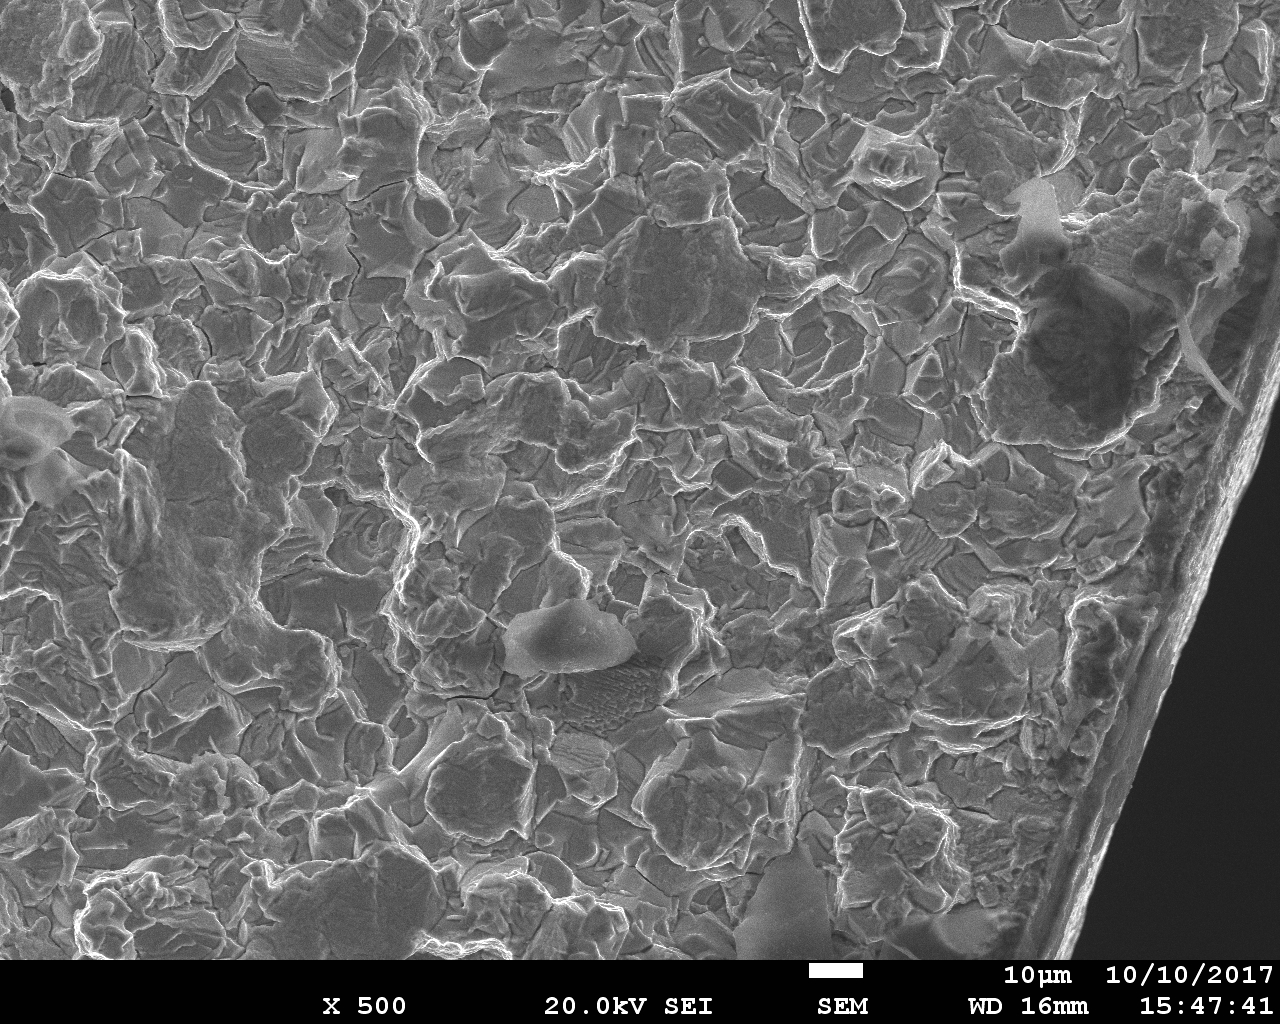
\includegraphics[width=6cm]{7206-2.jpg}
%     \centerline{(d)TC-IP-TGMF $\Delta \varepsilon_{eq}/2=0.55\%$.}
%   \end{minipage}%
%   \begin{minipage}[t]{0.5\linewidth}
%     \centering
%     \includegraphics[width=6cm]{730112.jpg}
%     \centerline{(c)TC-IP-TGMF-TBC $\Delta \varepsilon_{eq}/2=0.55\%$.}
%   \end{minipage}

%   \caption{Observation of fatigue striations on fractures surface.}
%   \label{Fig:MicrostructureofInconel718}
% \end{figure}

\section*{Acknowledgement:}

\bibliographystyle{unsrt}            % bibliography style
%\bibliographystyle{plain}            % bibliography style
\bibliography{bibliography}          % personal bibliography file

\end{document} 